\chapter{Исследовательская часть}

\section{Технические характеристики}

Технические характеристики устройства, на котором выполнялись замеры по времени:

\begin{itemize}
	\item Процессор: Apple M1 Pro \cite{m1}
	\item Оперативная память: 32 ГБайт.
	\item Операционная система: macOS Ventura 13.5.2. \cite{macOS}
\end{itemize}

При замерах времени ноутбук был включен в сеть электропитания и был нагружен только системными приложениями.

\section{Демонстрация работы программы}

На изображении \ref{img:demonstration} представлена иллюстрация работы разработанного программного продукта. 
Конкретно, демонстрируются результаты выполнения алгоритмов для вычисления расстояний Левенштейна и Дамерау~---~Левенштейна на примере двух строк: "кот" и "скат". 
Кроме того, на рисунке показываются матрицы, используемые алгоритмами, которые требуют промежуточные матрицы для выполнения расчетов.\clearpage
\begin{figure}[h]
	\centering
	\includegraphics[height=0.7\textheight]{img/example.png}
	\caption{Демонстрация работы программы при поиске расстояний Левенштейна и Дамерау~---~Левенштейна}
	\label{img:demonstration}
\end{figure}

\clearpage

\section{Временные характеристики}

Результаты эксперимента замеров по времени приведены в таблице.
Замеры проводились на одинаковых длин строк от 1 до 10 с шагом 1.
\begin{table}[ht]
	\small
	\begin{center}
		\begin{threeparttable}
		\caption{Замер по времени для строк, размер которых от 1 до 10}
		\label{tbl:time}
		\begin{tabular}{|c|c|c|c|c|}
			\hline
			& \multicolumn{4}{c|}{\bfseries Время, мкс} \\ \cline{2-5}
			& \multicolumn{1}{c|}{\bfseries Левенштейн}
			& \multicolumn{3}{c|}{\bfseries Дамерау-Левенштейн} \\ \cline{2-5}
			\bfseries Длина (символ) & \bfseries Итеративный & \bfseries Итеративный & \multicolumn{2}{c|}{\bfseries Рекурсивный} \\ \cline{4-5}
			& & & \bfseries Без кеша & \bfseries С кешом
			\csvreader{csv/time.csv}{}
			{\\\hline \csvcoli & \csvcolii & \csvcoliii & \csvcoliv & \csvcolv} \\
			\hline
		\end{tabular}			
		\end{threeparttable}
	\end{center}
\end{table}

Cравнение производится на основе данных, представленных в таблице \ref{tbl:time}. 
Данные для всех алгоритмов представлены на рисунке \ref{plt:time_01}. 
Данные для всех алгоритмов, не включая рекурсивный Дамерау~---~Левенштейна представлены на рисунке \ref{plt:time_02}

Из-за того, что у алгоритма поиска расстояния Дамерау~---~Левенштейна задействуется дополнительная операция, которая замедляет алгоритм - он оказывается медленнее алгоритма поиска расстояния Левенштейна.
Так же видно, что рекурсивный алгоритм очень быстро становится крайне не эффективным и непригодным к использованию.
\begin{figure}[h]
	\centering
	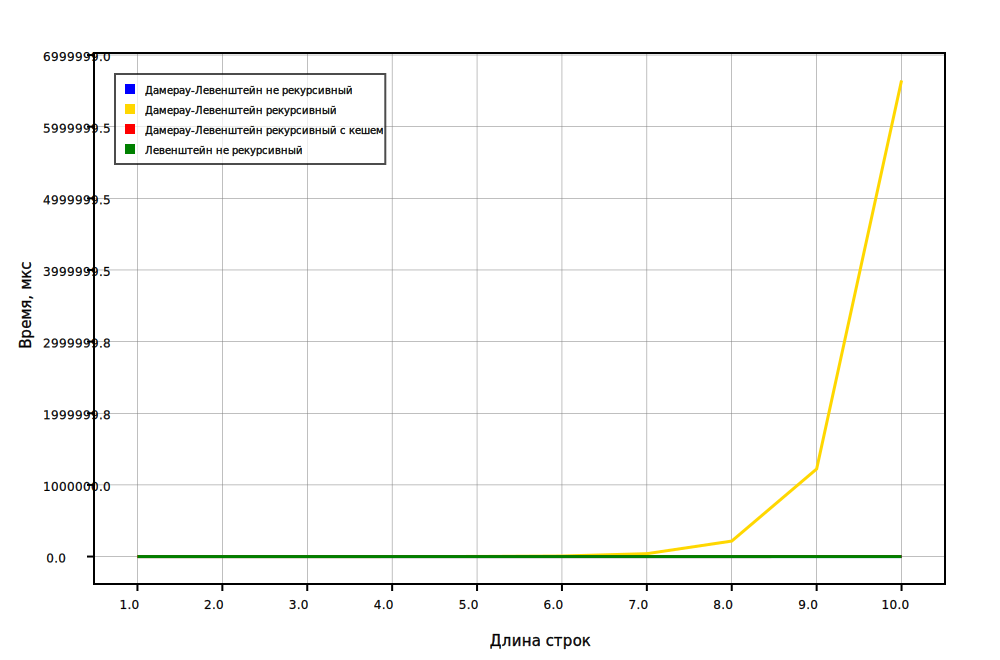
\includegraphics[height=0.4\textheight]{img/diag_02.pdf}
	\caption{Сравнение по времени реализаций алгоритмов поиска расстояний Левенштейна и Дамерау~---~Левенштейна}
	\label{plt:time_01}
\end{figure}

\begin{figure}[h]
	\centering
	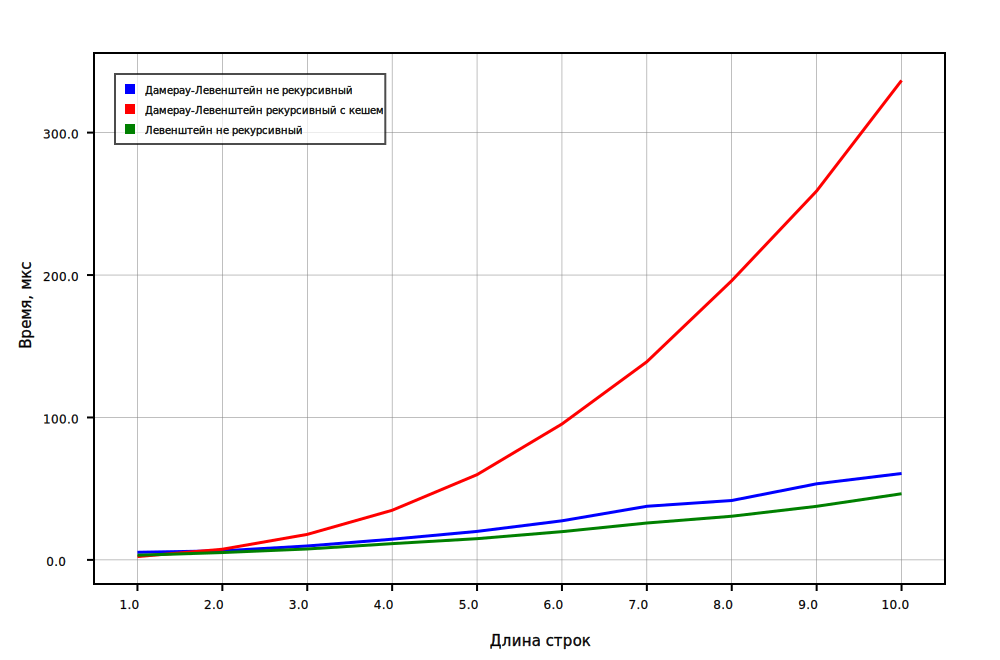
\includegraphics[height=0.4\textheight]{img/diag_01.pdf}
	\caption{Сравнение по времени реализаций алгоритмов без рекурсивного Дамерау~---~Левенштейна}
	\label{plt:time_02}
\end{figure}


\clearpage
\section{Характеристики по памяти}

Алгоритмы для вычисления расстояния Левенштейна и Дамерау--Левенштейна не различаются по потреблению памяти.
Максимальная глубина стека вызовов при использовании рекурсивной реализации равна сумме длин входных строк. 
Следовательно, максимальное использование памяти оценивается следующим образом:

\begin{equation}
(size(str1) + size(str2)) \cdot (8 \cdot size(Int) + size(Character))
\end{equation}

где $size$ - оператор, вычисляющий размер объекта, $str1$ и $str2$ - строки, $Character$ - тип данных для символов строки, и $Int$ - целочисленный тип.

В случае итеративной реализации потребление памяти теоретически можно оценить следующим образом:

\begin{equation}
	\begin{split}
(size(str1) + 1) \cdot (size(str2) + 1) \cdot size(Int) + 3\cdot size(Int) +\\
+ (n + m) \cdot size(Character).
	\end{split}
\end{equation}

\section{Вывод}

В данном разделе проведено сравнение затрат времени и памяти между алгоритмами вычисления расстояния Левенштейна и Дамерау -- Левенштейна. 
Наименее времязатратным оказался итеративный алгоритм для расчета расстояния Левенштейна.

Из собранных данных видно, что рекурсивная реализация алгоритма неэффективна на длинах строк, больших 5. 
Поэтому рекомендуется использовать рекурсивные алгоритмы только для строк малых размерностей (содержащих 1-4 символа).

Помимо этого, важно отметить, что алгоритм вычисления расстояния Дамерау~---~Левенштейна предпочтителен в случаях, когда возможны ошибки в транспозиции символов при печати текста, даже несмотря на его некоторое увеличение затрат по времени и памяти по сравнению с алгоритмом Левенштейна.

Рекурсивная реализация алгоритма для расчета расстояния Дамерау~---~Левенштейна требует больше времени по сравнению с итеративной реализацией.